\documentclass[12pt]{standalone}
\usepackage{tikz}
\usetikzlibrary{arrows.meta} % , decorations.pathreplacing}
% #problem([addition of paths])[ Suppose that points $x$ and $y$ in a topological space $X$ are joined by a path $phi.alt,$ 
% and points $y$ and $z$ are joined by a path $psi.$ Construct a path joining $x$ and $z.$]
% #solution[ Define a function $theta : [0,1] arrow.r X$ by
%$
%  theta\(t\) = cases(delim: "{",
%  // cases(delim: "{", 0\, & upright(" if ") x = y\,, 1\, & upright(" if ") x eq.not y .) 
%  phi.alt\(2t\) & upright(" if ") 0 lt.eq t lt.eq 1/2\,,
%  psi\(2t - 1\) & upright(" if ") 1/2 lt.eq t lt.eq 1\.
%  ) 
%$
%Since $phi.alt\(1\) = y = psi\(0\),$ the function $theta.alt$ is well-defined.
%Since $phi.alt$ and $psi$ are continuous, the function $theta.alt$ is continuous when restricted to the closed sets $[0,1/2]$ and $[1/2,1].$ 
%By the lemma about a function continuous on two closed sets, $theta$ is continuous on $[0,1],$ and so is a path joining $x$ and $z.$
%]
\begin{document}

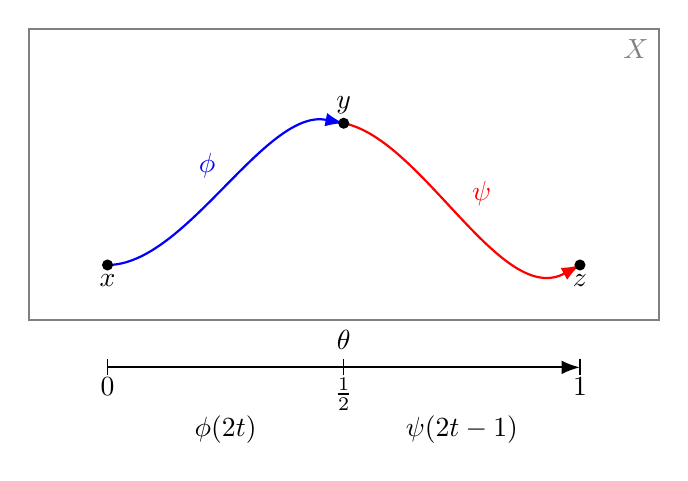
\begin{tikzpicture}% [yscale=0.8]
	\draw[thick, gray] (0, 0.8) rectangle (8, 4.5) node[anchor=north east] {$X$};

	\draw[thick, blue, -{Latex}]
		(1, 1.5) .. controls (2, 1.5) and (3, 3.5) .. (4, 3.3)
		node[midway, above left] {$\phi$};
	\draw[thick, red, -{Latex}]
		(4, 3.3) .. controls (5, 3.1) and (6, 0.95) .. (7, 1.5)
		node[midway, above right] {$\psi$};

	\fill (1, 1.5) circle (2pt) node[below] {$x$};
	\fill (4, 3.3) circle (2pt) node[above] {$y$};
	\fill (7, 1.5) circle (2pt) node[below] {$z$};

	\draw[thick, -{Latex}] (1, 0.2) -- (7, 0.2);
	\draw (1, 0.1) -- (1, 0.3) node[below=3pt] {$0$};
	\draw (4, 0.1) -- (4, 0.3) node[below=3pt] {$\frac12$};
	\draw (7, 0.1) -- (7, 0.3) node[below=3pt] {$1$};
	\node[below=14pt] at (2.5, 0.2) {$\phi(2t)$};
	\node[below=14pt] at (5.5, 0.2) {$\psi(2t-1)$};
	\node[above=3pt] at (4, 0.2) {$\theta$};
\end{tikzpicture}

\end{document}
